\begin{block}{ENSO, MJO, and Weather Types}
  \begin{mdframed}
  \begin{figure}
    \caption{
  		Anomalous probability of occurrence of each weather type concurrent with observance of each MJO and ENSO phase.
  		Only values which are significant at $p<0.10$ are shown.
      \label{fig:wt-mjo-enso}
  	}
  	\noindent\includegraphics[width=0.925\textwidth]{wt-mjo-enso.pdf}
  \end{figure}
  \end{mdframed}

  During El Ni\~{n}o years such as 2015-16, weather type 1 -- related to Chaco jet events -- occurs more frequently for almost all MJO phases, and particularly during phases 1, 2, and 5, consistent with observations of the year under study.
  This agreesß with previous studies \cite[i.e.][]{Velasco1987} which find that the intensity and exact location of the anomalous low-level anticylonic anomaly over central Brazil is relevant for the precise impact of ENSO events.

\end{block}
\begin{block}{Atlantic-Pacific Interaction and WT4}

  While the occurrence of WT1 during NDJF 2015-16 is well explained by ENSO and MJO variability, these features alone do not explain the occurrence of WT4, the ``No-Chaco'' jet event.
  Previous studies emphasize the importance of Pacific-Atlantic interaction for forecasting climate effects in this region \cite{Vera:2006ib,Barreiro:2017ct,Lima:2017hw,Munoz2015}.
  A persistent SST dipole in the central southern Atlantic Ocean favors the occurrence of WT4 by blocking transient extratropical wave activity coming from the Pacific, facilitating transitions from Chaco jet events (WT 1) to No-Chaco jet events (WT 4) via enhanced low-level wind circulation from southern Brazil towards the Atlantic, and back to north-east Brazil and the Amazon (see \cref{fig:chaco-nochaco}) due to land-sea temperature contrasts.
  Composite analysis (not shown) of months with many WT4 occurrences is consistent with the schematic shown here.

  \begin{mdframed}
  \begin{figure}
  	\noindent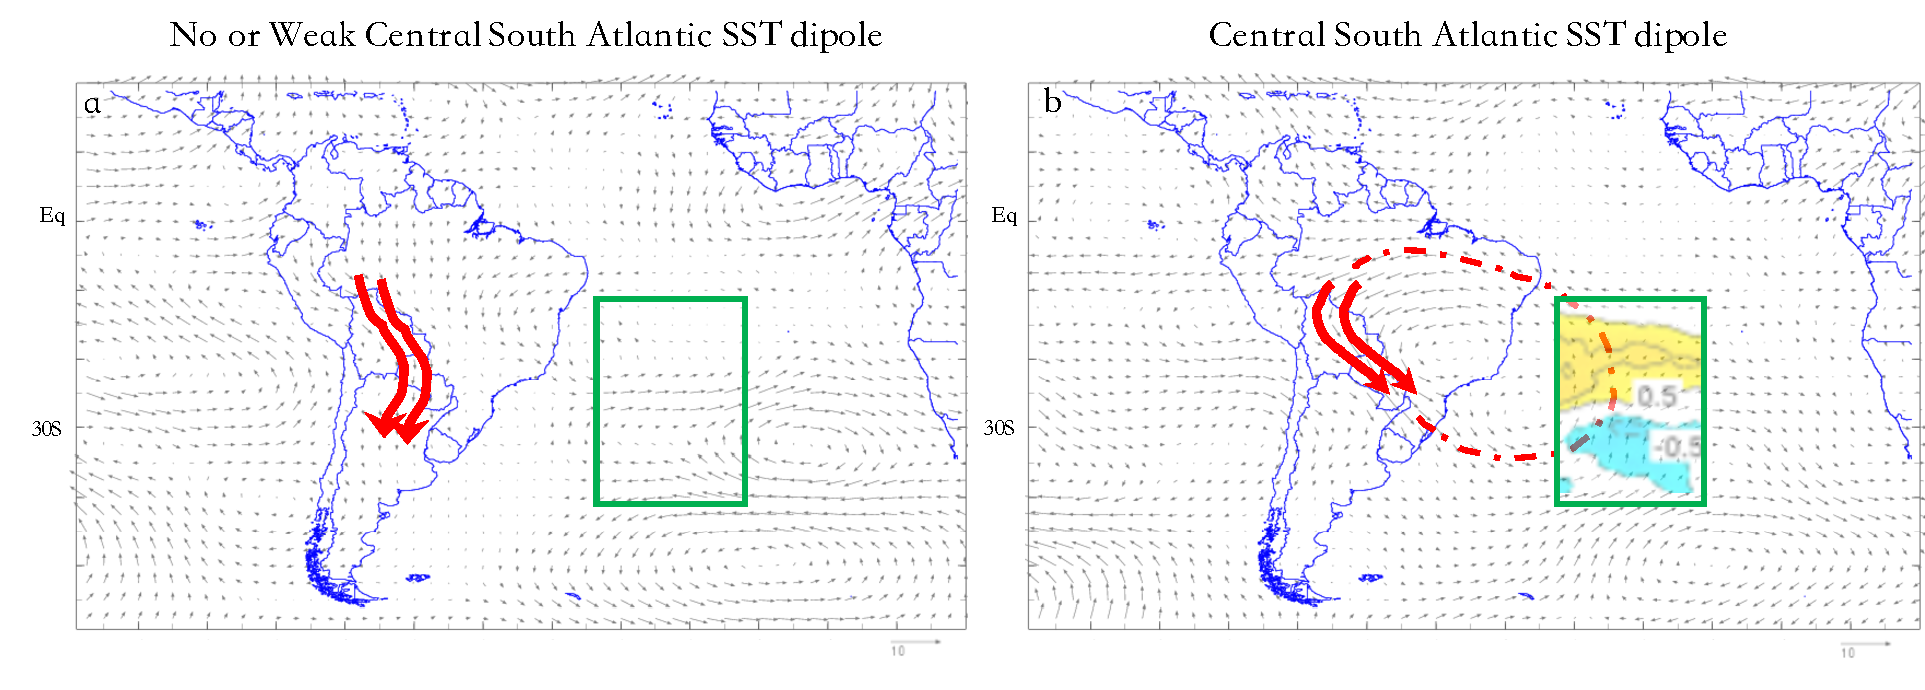
\includegraphics[width=0.925\textwidth]{../writeup/ChacoNoChacojet.pdf}
    \caption{
      Simple schematics of low-level jet events (red arrows) during austral summer and El Ni\~no years.
      \label{fig:chaco-nochaco}
  	}

  \end{figure}
  \end{mdframed}
\end{block}
